\documentclass[mat1]{fmfdelo}


% aktivirajte pakete, ki jih potrebujete
\usepackage{enumerate}
\usepackage{graphicx}

% za številske množice uporabite naslednje simbole
\newcommand{\R}{\mathbb R}
\newcommand{\N}{\mathbb N}
\newcommand{\Z}{\mathbb Z}
\newcommand{\C}{\mathbb C}
\newcommand{\Q}{\mathbb Q}
\newcommand{\PP}{\mathbb P}
\newcommand{\B}{\mathbb B}
\newcommand{\al}{\alpha}
\newcommand{\de}{\Delta}
\newcommand{\dd}{\textbf{d}}
\newcommand{\pp}{\textbf{p}}

% matematične operatorje deklarirajte kot take, da jih bo Latex pravilno stavil
\DeclareMathOperator{\conv}{conv}

% na razpolago so naslednja matematična okolja, ki jih kličemo s parom 
% \begin{imeokolja}[morebitni komentar v oklepaju] ... \end{imeokolja}
%
% definicija, opomba, primer, zgled, lema, trditev, izrek, posledica, dokaz
% 


% vstavite svoje definicije ...
%  \newcommand{}{}


% naslednje ukaze ustrezno napolnite
\avtor{Tjaša Bajc} 

\naslov{Geometrijska interpolacija štirih točk s parabolično krivuljo}
\title{Angleški prevod slovenskega naslova dela}

 \mentorica{izr.~prof.~dr.~Marjetka Knez}

\letnica{2018} % leto diplome

%  V povzetku na kratko opišite vsebinske rezultate dela. Sem ne sodi razlaga organizacije dela --
%  v katerem poglavju/razdelku je kaj, pač pa le opis vsebine.
\povzetek{}

%  Prevod slovenskega povzetka v angleščino. 
\abstract{}

% navedite vsaj eno klasifikacijsko oznako --
% dostopne so na www.ams.org/mathscinet/msc/msc2010.html
\klasifikacija{}
\kljucnebesede{} % navedite nekaj ključnih pojmov, ki nastopajo v delu
\keywords{} % angleški prevod ključnih besed


\begin{document}

%%%%%%%%%%%%%%%%%%%%%%%%%%%%%%%%%%%%%%%%%%%%%%%%%%%%%%%%%%%%%%%%%%%%%%%%%%%%%%%%%
% --------------------------------------------------------------------------------------------------------------------------------------------------------------------------------------------------------------------------
%%%%%%%%%%%%%%%%%%%%%%%%%%%%%%%%%%%%%%%%%%%%%%%%%%%%%%%%%%%%%%%%%%%%%%%%%%%%%%%%%

\section{Uvod}

Imamo štiri točke v ravnini. Zanima nas, kdaj lahko skoznje potegnemo parabolično krivuljo, to je parametrično polinomsko krivuljo stopnje dve, oziroma koliko je takih krivulj. Na primer, če so točke kolinearne, take prave paraboične krivulje očitno ne bomo našli. Kaj pa v ostalih primerih? Izkaže se, da je dovolj opazovati štirikotnik, katerega oglišča so dane točke. Pokazali bomo, da oglišča konveksnega štirikotnika, ki ni trapez, lahko interpoliramo z natanko dvema paraboličnima krivuljama, oglišča trapeza, ki ni paralelogram, pa z natanko eno parabolično krivuljo. V preostalih primerih štirih točk ne moremo interpolirati s parabolično krivuljo.


Poleg geometrijskega pristopa, ki smo ga na kratko povzeli zgoraj, se interpolacije lahko lotimo tudi z Lagrangeevimi baznimi polinomi. Vemo, da lahko štiri točke vedno interpoliramo s kubično krivuljo. Definirali bomo Lagrangeeve polinome stopnje tri in določili pogoje za proste parametre tako, da bo vodilni koeficient interpolacijskega polinoma enak $0$. Tako bomo dobili interpolacijsko polinomsko krivuljo stopnje dve, torej parabolično krivuljo.


V nadaljevanju si bomo ogledali še Hermitov problem. Namesto štirih točk bomo opazovali le dve, v katerih pa bomo poleg vrednosti predpisali tudi smer tangentnega vektorja. Poiskali bomo interpolacijsko krivuljo, ki bo zadoščala danim pogojem. Hermitov problem lahko posplošimo na več točk in opazujemo zlepke, ki jih dobimo z interpolacijo posameznih parov točk. Zlepek, ki ga dobimo na tak način, je geometrijsko zvezna krivulja, ki interpolira dane točke. 

Nazadnje bomo obravnavali aproksimacijo parametrično podanih krivulj s paraboličnimi krivuljami. Definirali bomo razdaljo med parametričnima krivuljama in opazovali konvergenco. Neformalno, opazovali bomo, kako hitro se parabolična krivulja približuje dani parametrični krivulji, ko aproksimiramo vedno manjši delček krivulje. Tabelirali bomo nekaj vrednosti in iz njih približno izračunali red konvergence. Izkaže se, da je v primeru aproksimacije s paraboličnimi krivuljami, red konvergence enak štiri, česar pa formalno ne bomo dokazali.

%%%%%%%%%%%%%%%%%%%%%%%%%%%%%%%%%%%%%%%%%%%%%%%%%%%%%%%%%%%%%%%%%%%%%%%%%%%%%%%%%
% --------------------------------------------------------------------------------------------------------------------------------------------------------------------------------------------------------------------------
%%%%%%%%%%%%%%%%%%%%%%%%%%%%%%%%%%%%%%%%%%%%%%%%%%%%%%%%%%%%%%%%%%%%%%%%%%%%%%%%%

\section{Geometrijska interpolacija}

V prvem razdelku se bomo interpolacijskega problema lotili geometrijsko. Za dane štiri točke v ravnini bomo iskali parabolično krivuljo, ki jih interpolira. Definirali bomo parabolično krivuljo kot množico točk v ravnini preko afinih matrik, opisali bomo kvadratično parametrizacijo parabolične krivulje in jo konkretno izračunali. Uvedli bomo baricentrične koordinate, navedli nekaj lastnosti in na koncu dokazali izrek, ki povezuje obstoj interpolacijske krivulje z obliko štirikotnika, katerega oglišča so dane točke. Konkretneje, dokazali bomo, da oglišč paralelograma ali konkavnega lika ne moremo interpolirati s parabolično krivuljo, oglišča trapeza lahko interpoliramo z natanko eno parabolično krivuljo, oglišča konveksnega štrirkotnika, ki ni trapez, pa z dvema takima krivuljama. Razdelek bomo zaključili s primerom konkretne interpolacijske naloge.

Za začetek definirajmo nekaj pojmov, ki jih bomo potrebovali v nadaljevanju.

\begin{definicija}
Naj bo $A'$ nesingularna $2\times2$ realna matrika, $d, e$ realni števili ter 
$$ A = 
\begin{bmatrix}
A' &
\begin{matrix}
0 \\
0
\end{matrix}
\\
\begin{matrix}
d & e
\end{matrix}
 & 1
\end{bmatrix}
.$$
Matriko $A$ imenujemo \emph{afina matrika}. 
\end{definicija}

% Ali tu rabimo kaj o grupi afinih matrik --- zaprtost za množenje, inverz,...?

Preko afinih matrik vpeljemo ekvivalenčno relacijo na množici realnih simetričnih $3 \times 3$ matrik.

\begin{definicija}
Matriki $B$ in $C$ sta \emph{afino podobni}, če obstaja afina matrika $A$, da velja $B = A C A^{T}$.
Da sta matriki afino podobni, označimo z $B \approx C$.
\end{definicija}

% Ali je to potrebno dokazati? Da je res EKV relacija?

\begin{definicija}\label{prva}
Definirajmo matriko 
$$D = 
\begin{bmatrix}
0 & 0 & 1 \\
0 & -2 & 0 \\
1 & 0 & 0
\end{bmatrix}.
$$
Definirajmo še podmnožico realnih simetričnih $3 \times 3$ matrik $$\PP = \{ B; B \approx d D, d \neq 0 \} .$$
\emph{Parabolična krivulja} je množica točk v ravnini 
\begin{equation}\label{implicitna}
 C_B = \{ (x,y); (x,y,1) B (x, y, 1)^T = 0, B \in \PP \}.
 \end{equation}
\end{definicija}

Če je matrika $B$ enaka $D$, je množica $C_B$ kar $C_B = \{ (x,y); x = y^2 \}$.

\begin{zgled}

(bom pripravila zgled: 

matriko $B$ in sliko parabole, ki jo podaja $C_B$)

\end{zgled}

Parabolično krivuljo lahko podamo v implicitni obliki kot v \eqref{implicitna} ali pa v parametrični obliki. Definirajmo kvadratično parametrizacijo parabolične krivulje, podane s $C_B$.

\begin{definicija}
Naj bodo $p(t)$, $q(t)$ in $r(t) \equiv 1$ linearno neodvisni polinomi stopnje največ dve. Če za nek $B$ iz množice $\PP$ velja 
$$ C_B = \{ (x,y); (x,y,1) B (x, y, 1)^T = 0 \} = \{ (p(t), q(t)); t \in \R \},$$
pravimo, da je $( p(t), q(t), 1)$ \emph{kvadratična parametrizacija} parabolične krivulje $C_B$.
\end{definicija}

Poglejmo, kako bi parametrično krivuljo zapisali v standardni bazi $t^2, t, 1$. Najprej bomo definirali matriko koeficientov, ki povezuje kvadratično parametrizacijo in zapis v standardni bazi, nato pa bomo pokazali, da lahko vsako parabolično krivuljo zapišemo v kvadratični parametrizaciji.

\begin{definicija}\label{defmatrikakoef}
Naj bodo $p(t)$, $q(t)$ in $r(t) \equiv 1$ linearno neodvisni polinomi stopnje največ dve. \emph{Matrika koeficientov $K$} je taka matrika, da velja $ (p(t), q(t), 1) = (t^2,t,1) K$.
\end{definicija} 

\begin{trditev}
Naj bodo $p(t)$, $q(t)$ in $r(t) \equiv 1$ linearno neodvisni polinomi stopnje največ dve, $K$ matrika koeficientov in $B \in \PP$. Tedaj velja
\begin{itemize}
\item $K$ je afina matrika,
\item  $ ( p(t), q(t), 1)$ je kvadratična parametrizacija za $C_B$ natanko tedaj, ko velja $K B K^T = d D$ za neki neničelni d.
\end{itemize}
\end{trditev}

% NOVO %%%%%%%%%%%%%%%%%%%%%%%%%%%%
\begin{dokaz}
Matrika $K$ je nesingularna, ker so $p(t), q(t)$ in 1 linearno neodvisni. Zadnja komponenta vektorja $(p(t), q(t), 1)$ je 1, torej mora biti zadnji stolpec matrike $K$ enak $(0,0,1)^T$. Sledi, da je matrika $K$ afina. Za dokaz druge točke trditve se spomnimo definicije kvadratične parametrizacije.
Velja:
\begin{align*}
0 &= (p(t), q(t), 1) B (p(t), q(t), 1)^T \\
   &= (t^2, t, 1) K B K^T (t^2, t, 1)^T \\
   &= (t^2, t, 1) 
\begin{bmatrix}
a & b & d \\
b & c & e \\
d & e & f
\end{bmatrix}
(t^2, t, 1)^T \\
   &= a t^4 + 2 b t^3 + (c+2d)t^2 + 2et + f
.\end{align*}
Zgornja enakost velja natanko tedaj, ko je $a=b=e=f=0$ in $c=-2d$. Tedaj je matrika $KBK^T$ oblike
$$
\begin{bmatrix}
0 & 0 & d \\
0 & -2d & 0 \\
d & 0 & 0
\end{bmatrix}
=
dD.
$$
\end{dokaz}

%%%%%%%%%%%%%%%%%%%%%%%%%%
Zgornja trditev ima dve koristni posledici. Najprej bomo dokazali, da lahko vsako parabolično krivuljo parametriziramo s kvadratično parametrizacijo, kasneje pa še, da različni matriki iz množice $\PP$ ne porodita nujno različnih paraboličnih krivulj.

\begin{posledica}\label{vsakaparabola}
Vsaka parabolična krivulja ima kvadratično parametrizacijo.
\end{posledica}

% NOVO %%%%%%%%%%%%%%%%%%%%%%%%%%%%
\begin{dokaz}
Res, saj smo parabolično krivuljo definirali kot
$$ C_B = \{ (x,y); (x,y,1) B (x, y, 1)^T = 0, B \in \PP \}.$$
Matrika $B$ je iz množice $\PP$, ki je definirana kot množica matrik, ki so afino podobne $D$. Matriko $B$ torej gotovo lahko zapišemo kot $ABA^T$ za neko afino matriko $A$. Po zgornji trditvi ima parabolična krivulja $C_B$ kvadratično parametrizacijo. Matrika koeficientov iz definicije \ref{defmatrikakoef} je tedaj matrika $A$.
\end{dokaz}
%%%%%%%%%%%%%%%%%%%%%%%%%%%%%

% NOVO %%%%%%%%%%%%%%%%%%%%%%%%%%%%

\begin{posledica}\label{bb*}
Naj bosta matriki $B$ in $\widetilde{B}$ elementa množice $\PP$. Enakost $C_B = C_{\widetilde{B}}$ velja natanko tedaj, ko velja $B = d \widetilde{B}$, $d \neq 0$.
\end{posledica}

\begin{dokaz}
%Dokaz je enostaven. 
Upoštevamo definicijo parabolične krivulje in hitro vidimo:
\begin{align*}
C_B    &= \{ (x,y); (x,y,1) B (x, y, 1)^T = 0\} \\
	&= \{ (x,y); (x,y,1) d \widetilde{B} (x, y, 1)^T = 0\} \\
	&= \{ (x,y); (x,y,1) \widetilde{B} (x, y, 1)^T = 0\} \\
	&= C_{\widetilde{B}}.
\end{align*}
\end{dokaz}
%%%%%%%%%%%%%%%%%%%%%%%%%%%%%

Interpolacije štirih točk s parabolično krivuljo se bomo lotili na naslednji način. Najprej bomo obravnavali tri točke in jih interpolirali. Izkazalo se bo, da v tem primeru dobimo družino parametrično podanih paraboličnih krivulj, torej, da interpolacijska krivulja še ni enolično določena. Nato bomo med krivuljami iz te družine poiskali tisto krivuljo, ki bo potekala tudi skozi četrto točko, seveda, če bo taka krivulja obstajala. Zato se najprej vprašajm, ali lahko vsako trojico različnih točk interpoliramo s parabolično krivuljo. Ne, hiter razmislek ali enostavna skica pokaže, da kolinearnih točk ne moremo interpolirati s parabolično krivuljo. Oglejmo si dokaz te trditve. 

\begin{trditev}
Različnih kolinearnih točk $T_0, T_1, T_2$ ne moremo interpolirati s parabolično krivuljo.
\end{trditev}

% NOVO %%%%%%%%%%%%%%%%%%%%%%%%%%%%

% Ta dokaz ni dobro napisan. Razmisli.

\begin{dokaz}
Vsako parabolično krivuljo lahko parametriziramo s $(t^2, t,1)K$ za neko afino matriko $K$. Izberimo tri različne vrednosti parametra $t$, iz katerih dobimo tri linearno neodvisne trojice $(t^2, t, 1)$. Ko vsako od teh trojic pomnožimo z matriko $K$, dobimo tri točke na paraboli, ki so gotovo nekolinearne, ker je $K$ afina matrika. Pokazali smo, da ne za nobene tri vrednosti parametra $t$ ne dobimo kolinearnih točk, torej ne moremo najti parabolične krivulje, ki bi potekala skozi kolinearne točke.
\end{dokaz}
%%%%%%%%%%%%%%%%%%%%%%%%%%%%%

Imejmo sedaj tri nekolinearne točke v ravnini $T_0, T_1, T_2$. Iščemo parabolično krivuljo $(p, q)$, ki bo pri nekih parametrih $t_0, t_1, t_2$ interpolirala dane točke, to je % JE TO PRAV ???
$$ T_0 = (p(t_0), q(t_0)), \qquad T_1 = (p(t_1), q(t_1)), \qquad T_2 = (p(t_2), q(t_2)).$$
Za parametre $t_0, t_1, t_2$ lahko zahtevamo $t_0 < t_1 < t_2$ in še dodatno $t_0 = 0$ in $t_2 = 1$. Za poljuben $t_1 \in (0,1)$  lahko najdemo taka $p(t), q(t)$ stopnje največ dve, da bo krivulja $ \{(p, q), t \in [0,1] \}$ rešila naš interpolacijski problem. Označimo $t_1$ z $\al.$  Polinoma $p$ in $q$  lahko dobimo z reševanjem sistema enačb
%
\begin{equation}\label{sistem1}
T_0 = (p(0), q(0)), \qquad T_1 = (p(\al), q(\al)), \qquad T_2 = (p(1), q(1)).
\end{equation}
%
Omenimo še, da je z izbiro $\al$ interpolacijska krivulja natanko določena, saj je zgornji sistem linearni sistem šestih enačb za šest neznank (koeficienti polinomov $p$ in $q$). Problem interpolacije štirih točk smo torej prevedli na iskanje take vrednosti parametra $\al$, da bo krivulja, ki jo določata polinoma $p$ in $q$, potekala skozi dano četrto točko. Ko bomo našli takšen $\al$, smo našli krivuljo, ki interpolira vse štiri dane točke v ravnini.
%
\begin{opomba}
Sistem \eqref{sistem1} je rešljiv za katerokoli število $\al$ iz $\R - \{ 0, 1\}$, a se zaradi urejenosti parametrov $t_0 = 0$, $t_1 = \al$ in $t_2 = 1$ omejimo na interval $(0, 1)$. Izbira $\al = 0$ ali $\al = 1$ očitno nima smisla, saj bi glede na sistem \eqref{sistem1} to pomenilo, da mora krivulja $(p, q)$ pri neki vrednosti parametra $t$ potekati skozi dve različni točki, kar je nemogoče.
\end{opomba}
%
Opazimo lahko, da dobimo pri drugačni vrednosti $\al$ drugo interpolacijsko krivujo. Dokler vrednosti parametra $\al$ ne fiksiramo, imamo torej družino paraboličnih krivulj, ki so sicer različnih oblik, a vse potekajo skozi točke $T_0, T_1$ in $T_2$. Povejmo to še formalno.

\begin{definicija}
Za nekolinearne točke $T_0, T_1, T_2$ naj bo $\B(T_0, T_1, T_2)$ množica vseh paraboličnih krivulj, ki potekajo skozi dane točke.
\end{definicija}

Naslednja trditev pokaže, da obstaja bijekcija med zgoraj definirano množico $\B(T_0, T_1, T_2)$ in množico $\R - \{0, 1\}$, torej, da za drug $\al$ dobimo drugačno parabolo, kot smo neformalno napisali že v opombi zgoraj.

\begin{trditev}
Za nekolinearne točke $(T_0, T_1, T_2)$ je preslikava, ki $\al$ priredi matriko $B_{\al}$, bijekcija med $\R - \{0, 1\}$ in množico $\B(T_0, T_1, T_2)$.
\end{trditev}

% NOVO %%%%%%%%%%%%%%%%%%%%%%%%%%%%


%\begin{opomba}
%V nadaljevanju bomo zaradi jasnosti uporabjlali krajše oznake, kadar bo iz konteksta jasno, katere so točke $T_0, T_1, T_2$. 
%\end{opomba}


\begin{dokaz}
Iz trditve \ref{parametrizacija} sledi, da za vsak $\al \in \R - \{0,1 \}$ parametrizacija $\Phi_\al(t)$ parametrizira neko parabolo $C_B$ iz množice $\B(T_0, T_1, T_2)$.
Obratno, zaradi posledice \ref{vsakaparabola} velja, da za vsako parabolo iz $\B(T_0, T_1, T_2)$ obstaja kvadratična parametrizacija, označimo jo s $\Psi(t)$.
Če za parametrizacijo $\Psi(t)$ velja, da je $\Psi(t_i) = (T_i, 1)$, postavimo $\al = \frac{t_1 - t_0}{t_2 - t_0}$.
Opazimo, da velja $\Phi_\al(t) = \Psi(t_0 + (t_2 - t_0)t)$ 
%. Od tod sledi
%\begin{align*}
%\Phi_\al(t_0) = \Psi(t_0 + (t_2 - t_0)t_0
, torej tudi $\Phi_\al$ parametrizira parabolo $C_B$. Sledi, da je $C_B$ element množice $\B(T_0, T_1, T_2)$ natanko tedaj, ko jo lahko parametriziramo s $\Phi_\al$ za nek $\al \in \R - \{0,1 \}$.
\end{dokaz}

% Ojoj !!!!!!!!!!!!!!!!!!!!!!!!!!!!!!!!!!!!!!!!!

% To

% tu

% moram

% še

% dobro

% razmislit.

%%%%%%%%%%%%%%%%%%%%%%%%%%%%%

Pokazali bomo, da lahko kvadratično parametrizacijo $(p(t), q(t),1)$ dobimo tudi drugače kot z dejanskim reševanjem sistema \eqref{sistem1}. Pred tem definirajmo še Vandermondovo matriko za naš primer, torej za parametre $t_0 = 0, t_1 = \al$ in $t_2 = 1$, in konfiguracijsko matriko za dane točke.

\begin{definicija}
Za realno število $\al$ definiramo \emph{Vandermondovo matriko} $V(\al)$,
$$V(\al) = 
\begin{bmatrix}
0 & 0 & 1 \\
\al ^2 & \al & 1 \\
1 & 1 & 1
\end{bmatrix}
.$$
Za točke v ravnini $T_0, T_1, T_2$ definiramo \emph{konfiguracijsko matriko}
$$R(T_0, T_1, T_2) = 
\begin{bmatrix}
T_0 & 1 \\
T_1 & 1 \\
T_2 & 1
\end{bmatrix}
.$$
\end{definicija}


\begin{trditev}\label{parametrizacija}
Naj bodo $T_0, T_1, T_2$  nekolinearne točke. Enolična kvadratična parametrizacija $\Phi_\al(t; T_0, T_1, T_2)$ krivulje, ki zadošča sistemu \eqref{sistem1}, je podana z naslednjim predpisom:
$$ \Phi_\al(t; T_0, T_1, T_2) = (t^2, t, 1) V(\al)^{-1} R(T_0, T_1, T_2).$$
\end{trditev}


% NOVO %%%%%%%%%%%%%%%%%%%%%%%%%%%%
\begin{opomba}
Inverz Vandermondove matrike v eksplicitni obliki je
$$
V(\al)^{-1} = 
\begin{bmatrix}
\frac{1}{\al} & \frac{1}{\al^2 - \al} & \frac{1}{1-\al} \\
- \frac{\al + 1}{\al} & \frac{1}{\al - \al^2} & \frac{\al}{\al-1} \\
1 & 0 & 0
\end{bmatrix}
.$$
\end{opomba}
%%%%%%%%%%%%%%%%%%%%%%%%%%%%%

% NOVO %%%%%%%%%%%%%%%%%%%%%%%%%%%%
\begin{dokaz}
Označimo najprej $T_0 = (x_0, y_0), T_1 = (x_1, y_1), T_2 = (x_2, y_2)$. Računamo:
%$$
\begin{align*}
%%$$
\Phi_\al(t; T_0, T_1, T_2) &=  (t^2, t, 1) V(\al)^{-1} R(T_0, T_1, T_2) \\
				&=  (t^2, t, 1)  
\begin{bmatrix}
\frac{1}{\al} & \frac{1}{\al^2 - \al} & \frac{1}{1-\al} \\
- \frac{\al + 1}{\al} & \frac{1}{\al - \al^2} & \frac{\al}{\al-1} \\
1 & 0 & 0
\end{bmatrix}
\begin{bmatrix}
x_0 & y_0 & 1 \\
x_1 & y_1 & 1 \\
x_2 & y_2 & 1 
\end{bmatrix}
\\
				&= \frac{1}{\al^2 - \al} 
\begin{bmatrix}
t^2(\al - 1) - t(\al^2 - 1) + \al(\al - 1) \\
 t^2 - t \\
\al t(\al - t)
\end{bmatrix}
^T
\begin{bmatrix}
x_0 & y_0 & 1 \\
x_1 & y_1 & 1 \\
x_2 & y_2 & 1 
\end{bmatrix}
.\\
\end{align*}
Ko rezultat uredimo, dobimo naslednje: 
$$ 
\begin{bmatrix}
t^2 ( \frac{x_0}{\al} + \frac{x_1}{\al^2 - \al} - \frac{x_2}{\al -1} ) + t(- \frac{x_0(\al + 1)}{\al} - \frac{x_1}{\al^2 - \al} + \frac{x_2 \al}{\al - 1}) + x_0 \\
t^2 ( \frac{y_0}{\al} + \frac{y_1}{\al^2 - \al} - \frac{y_2}{\al -1} ) + t(- \frac{y_0(\al + 1)}{\al} - \frac{y_1}{\al^2 - \al} + \frac{y_2 \al}{\al - 1}) + y_0 \\
1
\end{bmatrix}
^T
= (p(t), q(t), 1).
$$
Preverimo, da polinom $p$ ustreza trditvi, torej da interpolira prve koordinate točk $T_0, T_1, T_2$. Res:
\begin{align*}
p(0) &= x_0, \\
p(\al) &= x_0 \al  + \frac{x_1 \al }{\al - 1} - \frac{x_2 \al^2 }{\al - 1} - x_0(\al + 1) - \frac{x_1}{\al - 1} + \frac{ x_2 \al^2}{\al - 1} + x_0 = x_1, \\
p(1) &= \frac{x_0}{\al} + \frac{x_1}{\al^2 - \al} - \frac{x_2}{\al -1} - \frac{x_0(\al + 1)}{\al} - \frac{x_1}{\al^2 - \al} + \frac{x_2 \al}{\al - 1} + x_0 = x_2.
\end{align*}
Analogno velja za polinom $q$, torej smo res našli kvadratično parametrizacijo interpolacijske krivulje.
\end{dokaz}
%%%%%%%%%%%%%%%%%%%%%%%%%%%%%

Spomnimo se definicije parabolične krivulje \ref{prva}. V definiciji nastopi matrika $B$ iz množice $\PP$. Kasneje smo povedali, da ima vsaka tako definirana krivulja kvadratično parametrizacijo $(p(t), q(t), 1)$. Trditev \ref{parametrizacija} nam da parametrizacijo krivulje, ki poteka skozi točke $T_0, T_1$ in $T_2$. Katera pa je tista matrika $B$ iz definicije \ref{prva}, ki porodi to krivuljo? Očitno bo ta matrika odvisna tudi od vrednosti parametra $\al$, zato jo bomo označili z $B_\al$. 
%
\begin{definicija}\label{aalfa}
Definiramo matriki

$$A_{\al} = V(\al) \ D \ V(\al)^T $$
in
$$B_{\al} =  R(T_0, T_1, T_2)^{-1}\  A_{\al} \  (R(T_0, T_1, T_2)^{-1})^T.$$
\end{definicija}

\begin{opomba}
Matriko $A_\al$ enostavno izračunamo in zapišemo eksplicitno z % JE z RES OK?
$$A_\al = 
\begin{bmatrix}
0 & \al^2 & 1 \\
\al^2 & 0 & (\al - 1)^2 \\
1 & (\al -1)^2 & 0
\end{bmatrix}
.$$

\end{opomba}
%
Na začetku razdelka smo napovedali izrek, ki bo povezal obliko štirikotnika z obstojem parabolične krivulje, ki interpolira njegova oglišča. Ker je pomembna oblika štirikotnika, bi želeli nekako opisati relativni položaj četrte točke glede na prve tri. Na primer, želeli bi na enostaven način preveriti, ali recimo leži četrta točka znotraj ali zunaj trikotnika, katerega oglišča so prve tri točke. Iz tega bomo lahko sklepali o konveksnosti ali konkavnosti lika. Vpeljimo torej baricentrične koordinate točke $T_3$ glede na točke $T_0, T_1$ in $T_2$.

\begin{definicija}
Za dane nekolinearne točke $T_0, T_1, T_2$ definiramo \emph{vektor baricentričnih koordinat} $b = (b_0, b_1, b_2)$, da za neko četrto točko $T_3$ velja
% SPREMENJENO; DODANA VSOTA
\begin{align*}
(T_3, 1) &= \sum_{i=0}^{2} b_i (T_i, 1) \\
	   & = b R(T_0, T_1, T_2).
	   \end{align*}
% KONEC SPREMEMBE 
\end{definicija}
Sledi $ b = (T_3, 1) R(T_0, T_1, T_2)^{-1}$.
Nekaj lastnosti tako definiranega vektorja $p$ podaja spodnja trditev.

\begin{trditev}\label{vektorp}
Za zgoraj definiran $b$ velja $b_0 + b_1 + b_2 = 1$ in $b_i = 0$ natanko tedaj, ko točka $T_3$ leži na isti premici kot točki $T_j$ in $T_k$, $i, j, k \in \{0, 1, 2 \}, i \neq j, j\neq k, i \neq k$. 
\end{trditev}

% NOVO %%%%%%%%%%%%%%%%%%%%%%%%%%%%
\begin{dokaz}

Dovolj je dokazati, da velja $b_0 = 0$ in $b_2 = 1 - b_1$ natanko tedaj, ko točka $T_3$ leži na isti premici kot točki $T_1$ in $T_2$.
Vektor $b$ je v tem primeru enak $(0, b_1, 1 - b_1)$. Glede na definicijo baricentričnih koordinat velja
$$(T_3, 1) = (x_3, y_3, 1) = (b_1 x_1 + (1 - b_2)x_2, b_1 y_1 + (1 - b_2) y_2, 1).$$
Premica, ki poteka skozi točki $T_1$ in $T_2$, je podana z enačbo
$$ y = \frac{y_2 - y_1}{x_2 - x_1} x + \frac{x_2 y_1 - x_1 y_2}{x_2 - x_1} .$$
Z enostavnim računom se prepričamo, da točka $T_3$ leži na tej premici.

\end{dokaz}
%%%%%%%%%%%%%%%%%%%%%%%%%%%%%

Označimo sedaj s $T = \{T_0, T_1, T_2, T_3 \}$ nabor štirih točk v ravnini, od katerih nobene tri niso kolinearne. Take točke so oglišča konveksnega štirikotnika, če nobena točka $T_i$ ni v konveksni lupini preostalih treh točk, torej znotraj trikotnika, katerega oglišča so preostale tri točke.

\begin{trditev}\label{konveks}
Točke iz $T$ so oglišča konveksnega štirikotnika natanko tedaj, ko velja $b_0 b_1 b_2 < 0$, kjer so $b_0, b_1, b_2$ komponente vektorja $b$, za katerega velja $(T_3, 1) = b R(T_0, T_1, T_2).$
\end{trditev}

% NOVO %%%%%%%%%%%%%%%%%%%%%%%%%%%%
\begin{dokaz}

% Ne znam.

\end{dokaz}
%%%%%%%%%%%%%%%%%%%%%%%%%%%%%

Sedaj lahko zapišemo glavni izrek prvega razdelka.

\begin{izrek}\label{glavniizrek}
Naj bo $T = \{ T_0, T_1, T_2, T_3 \}$ nabor štirih točk v ravnini, od katerih nobene tri niso kolinearne.

\begin{enumerate}[i)]

\item Če so točke iz $T$ oglišča konkavnega štirikotnika, danih točk ne moremo interpolirati s parabolično krivuljo.

\item Če so točke iz $T$ oglišča paralelograma, danih točk ne moremo interpolirati s parabolično krivuljo.

\item Če so točke iz $T$ oglišča trapeza, ki ni paralelogram, lahko dane točke interpoliramo z natanko eno parabolično krivuljo.

\item Če so točke iz $T$ oglišča konveksnega štirikotnika, ki ni trapez, lahko dane točke interpoliramo z natanko dvema paraboličnima krivuljama.
\end{enumerate}

\end{izrek}

\begin{dokaz}
Najprej bomo poiskali družino interpolacijskih krivulj za prve tri točke $T_0, T_1$ in $T_2$ in jo označili z  $\B(T_0, T_1, T_2)$. Zaenkrat je parameter $\al$ še prost. Spomnimo se matrik $A_\al$ in $B_\al$ iz definicije \ref{aalfa}. Četrta točke $T_3$ leži na neki parabolični krivulji iz množice $\B(T_0, T_1, T_2)$ natanko tedaj, ko obstaja tak $\al \in \R - \{0,1 \}$, da točka $T_3$ leži na $C_{B_\al}$. Po definiciji \ref{implicitna} točka leži na parabolični krivulji natanko tedaj, ko velja
%
\begin{align}
0	&= (T_3, 1) B_\al (T_3, 1)^T \nonumber \\
	&= (T_3, 1) R(T_0, T_1, T_2)^{-1}\  A_{\al} \  (R(T_0, T_1, T_2)^{-1})^T (T_3, 1)^T \nonumber \\
	&= (b_0, b_1, b_2) A_\al (b_0, b_1, b_2)^T \nonumber \\
	&= \al^2 b_0 b_1 + (\al - 1)^2 b_1 b_2 + b_0 b_2 \label{14} \\ % Spustimo 2 - lahko izpostavimo iz vseh členov
	&= \al^2 b_1(b_0 + b_2) - 2 \al b_1 b_2 + b_2(b_0 + b_1). \label{15}
\end{align}
Dobili smo kvadratno enačbo za $\al$, katere diskriminanta je 
\begin{align*}
D	&= 4 b_1^2 b_2^2 - 4 b_1 b_2(b_0 + b_2)(b_0 + b_1)  \\
	&= 4 b_1 b_2(b_1 b_2 - (1 - b_1)(1 - b_2))  \\
	&= 4 b_1 b_2(b_1 b_2 - 1 + b_1 + b_2 - b_1 b_2)  \\
	&= - 4 b_0 b_1 b_2. 
\end{align*}
Upoštevali smo, da velja $ b_0 + b_1 + b_2 = 1$. Produkt $b_0 b_1 b_2$ je različen od nič, saj nobene tri točke niso kolinearne. Obravnavajmo sedaj rešitve enačbe \eqref{15} glede na to, koliko baricentričnih koordinat točke $T_3$ je enakih 1.

Najprej naj bosta dva od $b_0, b_1, b_2$ enaka $1$, tretji pa $-1$. Preverimo vsako od možnosti. Za $b_0 = -1$ dobimo rešitev $\al = 0$, za $b_1 = -1$ dobimo $\al(1 - \al) = 0$, torej je $\al = 0$ ali $\al = 1$, za $b_2 = -1$ pa dobimo rešitev $\al = 1$. V nobenem od primerov se točk torej ne da interpolirati s parabolično krivuljo. Izkaže se, da v primeru, da sta dve baricentrični koordinati enaki $1$, dane štiri točke tvorijo oglišča paralelograma.

Sedaj naj bo natanko ena od baricentričnih koordinat enaka $1$. Drugi dve se v tem primeru razlikujeta le za predznak. Spet poračunamo vse tri možnosti in dobimo naslednje rezultate:
\begin{itemize}
\item če je $b_0 = 1$, je rešitev $\al = \frac{b_1 + 1}{b_1 - 1} = \frac{b_2 - 1}{b_2 + 1}$,
\item če je $b_1 = 1$, je rešitev $\al = \frac{b_0 + 1}{2} = \frac{1 - b_2}{2}$,
\item če je $b_2 = 1$, je rešitev $\al = \frac{2}{b_0 + 1} = \frac{2}{1 - b_2}$.
\end{itemize}
Vidimo, da v vseh primerih dobimo natanko eno rešitev, torej natanko eno interpolacijsko krivuljo. Če je natanko ena od baricentričnih koordinat enaka $1$, so dane štiri točke oglišča trapeza.

%Opazimo naslednje:
%\begin{enumerate}[a)]
%\item enačba \eqref{15} ima enolično rešitev natanko tedaj, ko je $b_1 = 1$,
%\item $\al = 0$ je ena od rešitev enačbe \eqref{15} natanko tedaj, ko je $b_2 = 1$, % druga rešitev je \al = \frac{2}{p_0 + 1}
%\item $\al = 1$ je ena od rešitev enačbe \eqref{14} natanko tedaj, ko je $b_0 = 1$, % druga rešitev je \al = \frac{p_2 - 1}{p_2 + 1}
%\end{enumerate}
%
%Če sta dva od parametrov $b_0, b_1, b_2$ enaka $1$, je rešitev enačbe \eqref{15} bodisi $\al = 0$ bodisi $\al = 1$. V tem primeru ne obstaja interpolacijska parabolična krivulja za dane točke. Izkaže se, da so tem primeru točke iz $T$ oglišča paralelograma.
%
%Če je natanko en od parametrov $b_0, b_1, b_2$ enak $1$, ima enačba \eqref{15} natanko eno rešitev. Natančneje, 
%\begin{itemize}
%\item če je $b_0 = 1$, je rešitev $\al = \frac{b_1 + 1}{b_1 - 1} = \frac{b_2 - 1}{b_2 + 1}$,
%\item če je $b_1 = 1$, je rešitev $\al = \frac{b_0 + 1}{2} = \frac{1 - b_2}{2}$,
%\item če je $b_2 = 1$, je rešitev $\al = \frac{2}{b_0 + 1} = \frac{2}{1 - b_2}$.
%\end{itemize}
%V tem primeru so točke iz $T$ oglišča trapeza, ki ni paralelogram.

Če so vse vrednosti parametrov $b_0, b_1, b_2$ različne od $1$, točke iz $T$ niso oglišča trapeza. Iz posledice \ref{konveks} sledi, da so točke iz $T$ oglišča konveksnega štirikotnika natanko tedaj, ko je $b_0 b_1 b_2 < 0$, kar pomeni, da je diskriminanta enačbe \eqref{15} strogo pozitivna in obstajata dve različni rešitvi. To sta
\begin{equation*}
\al_{1,2} = \frac{b_1 b_2 \pm \sqrt{b_0 b_1 b_2}}{b_1 ( b_0 + b_2)}.
\end{equation*}
Tedaj lahko točke iz $T$ interpoliramo z dvema različnima paraboličnima krivuljama.

Enačba \eqref{15} nima rešitve, če je njena diskriminanta negativna. Kot zgoraj je to natanko tedaj, ko so točke iz $T$ oglišča konkavnega štirikotnika.
\end{dokaz}

Konkreten interpolacijski problem rešimo tako, da izračunamo vektor $b$ iz trditve \ref{vektorp}, iz njegovih komponent pa izračunamo ustrezen $\al$ kot v dokazu zgoraj. Parametrizacijo krivulje -- torej polinoma $p$ in $q$ -- smo eksplicitno zapisali v dokazu trditve \ref{parametrizacija}, za implicitno obliko parabolične krivulje $C_{B_\al}$ pa izračunamo še matriki $A_\al$ in $B_\al$ iz definicije \ref{aalfa}.
%
\begin{primer}
Dane so točke $T_0 = (0, 2), T_1 = (-1, -1)$ in $T_2 = (3, -1).$
Tem točkam dodamo še četrto točko $T_3$. Iz zgornjega izreka sledi, da dobljenih štirih točk ne bo mogoče interpolirati s parabolično krivuljo v primeru, da bodo tvorile konkaven lik ali paralelogram. 
%
\begin{figure}[h!]
  \centering
      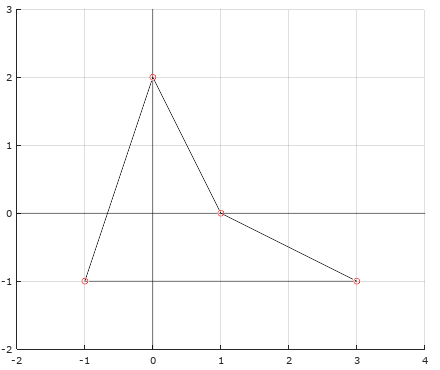
\includegraphics[width=0.65\textwidth]{okonk.png}
  \caption{Oglišč konkavnega lika ne moremo interpolirati s parabolično krivuljo.}
  \label{fig:slikakonk}
\end{figure}
%
\begin{figure}[h]
  \centering
      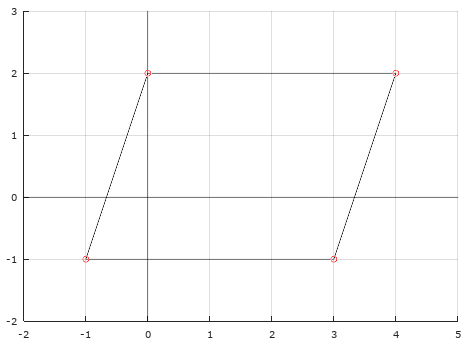
\includegraphics[width=0.65\textwidth]{opara.png}
  \caption{Tudi paralelograma ne moremo interpolirati s parabolično krivuljo.}
  \label{fig:slikapara}
  \end{figure}
%
Na sliki \ref{fig:slikakonk} smo prvim trem točkam dodali točko $(1,0)$ in tako dobili konkaven lik, na sliki \ref{fig:slikapara} pa točko $(4,2)$ in dobili paralelogram. V nobenem primeru oglišč ne moremo interpolirati s parabolično krivuljo. Na sliki \ref{fig:slikatrap} smo danim trem točkam dodali točko $(-1/2, - 3/2)$. Skupaj s prejšnjimi točkami tvori oglišča trapeza in zato obstaja natanko ena parabolična krivulja $(p(t), q(t))$, ki jih interpolira. Na sliki je narisan del krivulje za vrednosti $t$ med $0$ in $1$.
%
\begin{figure}[h!]
  \centering
      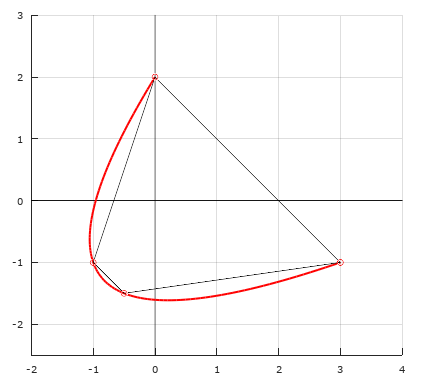
\includegraphics[width=0.65\textwidth]{otrap}
  \caption{Oglišča trapeza interpolira natanko ena parabolična krivulja.}
  \label{fig:slikatrap}
  \end{figure}
%
Za točke na sliki \ref{fig:slikatrap} velja $(p(0), q(0)) = (0,2) = T_0$ in $(p(1), q(1)) = (3, -1) = T_2$. Kaj pa parameter $\al$, za katerega velja $p(\al), q(\al)) = (-1, 0) = T_1$? Izkaže se, da je za točke $T_0, T_1$ in $T_2$ vektor baricentričnih koordinat $b$ iz trditve \ref{vektorp} enak $(-1/6, 1, 1/6)$. Iz dokaza izreka \ref{glavniizrek} preberemo, da je $\al = \frac{b_0 + 1}{2} = 5/12$. Zapišimo še eksplicitno polinoma $p$ in $q$ s pomočjo trditve \ref{parametrizacija}:
%
\begin{align*}
p(t) &= t^2 ( \frac{x_0}{\al} + \frac{x_1}{\al^2 - \al} - \frac{x_2}{\al -1} ) + t(- \frac{x_0(\al + 1)}{\al} - \frac{x_1}{\al^2 - \al} + \frac{x_0 \al}{\al - 1}) + x_0 \\
       &= t^2 \frac{324}{35} - t \frac{219}{35}, \\
q(t) &= t^2 ( \frac{y_0}{\al} + \frac{y_1}{\al^2 - \al} - \frac{y_2}{\al -1} ) + t(- \frac{y_0(\al + 1)}{\al} - \frac{y_1}{\al^2 - \al} + \frac{y_0 \al}{\al - 1}) + y_0  \\
       &= t^2 \frac{36}{5} - t \frac{51}{5} + 2.
\end{align*}
Parabolično krivuljo smo uvodoma definirali kot množico točk v ravnini preko matrike $B_\al$. Oglejmo si še, kako izgleda v našem primeru ta matrika, ki jo dobimo kar iz definicije \ref{aalfa}:
%
\begin{align*}
 B_{5/12} &= R(T_0, T_1, T_2)^{-1}\  A_{5/12} \  (R(T_0, T_1, T_2)^{-1})^T \\
 	      &= 
\begin{bmatrix}
0 & -1/4 & 1/4 \\
1/3 & -1/4 & -1 \\
1/3 & 1/2 & 1/6
\end{bmatrix}
\begin{bmatrix}
0 & 25/144 & 1 \\
25/144 & 0 & 49/144 \\
1 & 49/144 & 0
\end{bmatrix}
\begin{bmatrix}
0 & 1/3 & 1/3 \\
-1/4 & -1/4 & 1/2 \\
1/4 & -1 & 1/6
\end{bmatrix}
\\
	& = \frac{1}{1152}
	\begin{bmatrix}
-49 & 63 & 112 \\
63 & -81 & 16 \\
112 & 16 & 260
\end{bmatrix}.
 \end{align*}
 %
 Interpolacijska parabolična krivulja za oglišča trapeza $T_0 = (0, 2)$, $T_1 = (-1,-1)$, $T_2 = (3, -1)$ in $T_3 = (-1/2, -3/2)$ je torej $ C_{B_{5/12}} = \{ (x,y); (x,y,1) B_{5/12} (x, y, 1)^T = 0 \}$. Njena kvadratična parametrizacija je $(p(t), q(t),1)$, kjer sta $p$ in $q$ zgoraj iz\-ra\-ču\-na\-na polinoma.
\end{primer}

%%%%%%%%%%%%%%%%%%%%%%%%%%%%%%%%%%%%%%%%%%%%%%%%%%%%%%%%%%%%%%%%%%%%%%%%%%%%%%%%%
% --------------------------------------------------------------------------------------------------------------------------------------------------------------------------------------------------------------------------
%%%%%%%%%%%%%%%%%%%%%%%%%%%%%%%%%%%%%%%%%%%%%%%%%%%%%%%%%%%%%%%%%%%%%%%%%%%%%%%%%


\section{Interpolacija z Lagrangeevimi baznimi polinomi}

V tem razdelku si bomo ogledali rešitev interpolacijskega problema na bolj algebraičen način. Vemo, da lahko štiri točke interpoliramo s kubično krivuljo. Interpolacijsko krivuljo bomo zapisali z Lagrangeevimi baznimi polinomi, kar bo enostavneje, kot če bi delali v standardni bazi. Nato bomo reševali sistem enačb, ki ga dobimo, ko vodilni koeficient polinoma v Lagrangeevi bazi izenačimo z nič, s čimer znižamo stopnjo s tri na dve. Definirajmo najprej interpolacijski problem.

Za dane točke $T_i$ v ravnini, $i = 0, 1, 2, 3$, iščemo parabolično krivuljo $\textbf{p} : [ 0, 1 ] \rightarrow \R^2$, da bo veljalo $$\textbf{p}(t_i) = T_i, \qquad i = 0, 1, 2, 3.$$ 

Dodatno zahtevamo, da so parametri urejeni, torej $t_0 < t_1 < t_2 < t_3$. Brez škode za splošnost lahko postavimo $t_0 = 0$ in $t_3 = 1$.

Definirajmo Lagrangeeve bazne polinome najprej v splošnem, kasneje pa bomo konkretno zapisali tiste, ki jih bomo potrebovali pri reševanju našega problema, torej polinome stopnje tri.

\begin{definicija}
\emph{Lagrangeeve bazne polinome} stopnje $n$ definiramo
%
$$ \ell_{i,n}(t) = \prod_{\substack{j=0 \\ j \neq i}}^{n} \frac{t - t_j}{t_i - t_j} , \qquad i = 0, 1, \ldots n.$$	
\end{definicija}
%
Lagrangeevi bazni polinomi so vsi stopnje $n$. Poleg tega zanje velja $$\ell_{i,n}(t_j) = \delta_{ij}.$$
% N O V O 
Omenimo še, da tvorijo Lagrangeevi bazni polinomi particijo enote. Velja torej naslednje
%
\begin{equation*}
\sum_{i = 0}^{n} \ell_{i,n}(t) = 1.
\end{equation*}
%
Oglejmo si polinome $ \ell_{0,3}(t), \ell_{1,3}(t), \ell_{2,3}(t)$ in $ \ell_{3,3}(t) $, ki so baza za prostor polinomov tretje stopnje:
%
\begin{align*}
	\ell_{0,3}(t) &= \frac{(t - t_1)(t - t_2)(t - t_3)}{(t_0 - t_1)(t_0 - t_2)(t_0 - t_3)}, \\
	\ell_{1,3}(t) &= \frac{(t - t_0)(t - t_2)(t - t_2)}{(t_1 - t_0)(t_1 - t_2)(t_1 - t_3)}, \\
	\ell_{2,3}(t) &= \frac{(t - t_0)(t - t_1)(t - t_3)}{(t_2 - t_0)(t_2 - t_1)(t_2 - t_3)}, \\
	\ell_{3,3}(t) &= \frac{(t - t_0)(t - t_1)(t - t_2)}{(t_3 - t_0)(t_3 - t_1)(t_3 - t_2)}. 	
\end{align*}

Interpolacijsko krivuljo lahko razvijemo po Lagrangeevih baznih polinomih kot 
\begin{equation}\label{razvoj}
p(t) = \sum_{i=0}^{3} a_i \ell_{i,n}(t),
\end{equation}
%
kjer so $a_i \in \R$ neznani koeficienti.

Hitro lahko vidimo, kaj so koeficienti $a_i$ pri interpolacijskem polinomu. Uvodoma smo zapisali, da naj za $\textbf{p}$ velja, da je $\textbf{p}(t_j) = T_j$. Ko vstavimo $t_j$ v \eqref{razvoj}, dobimo
\begin{align*}
\textbf{p}(t_j) &=  \sum_{i=0}^{3} a_i \ell_{i,n}(t_j) \\
	 &= \sum_{i=0}^{3} a_i \delta_{ij} \\
	&= a_j
,\end{align*}
od koder sledi, da so iskani koeficienti kar točke, ki jih interpoliramo. Interpolacijski polinom v Lagrangeevi obliki torej zapišemo kot 
$$\textbf{p}(t) = \sum_{i=0}^{3} T_i \ell_{i,n}(t).$$

Spomnimo, da so polinomi $\ell_{i,n}$ stopnje tri. Ker iščemo parabolično krivuljo, mora biti vodilni koeficient enak nič. To nam da nelinearen sistem
\begin{equation}\label{vodkoef}
\sum_{i = 0}^{3} \frac{T_i}{\prod_{\substack{j = 0 \\ j \neq i}}^3(t_i - t_j)} = 0
\end{equation}
%
za neznana parametra $t_1$ in $t_2$, enačbi pa dobimo iz komponent \eqref{vodkoef}, saj so $T_i$ točke v ravnini.
%
% N O V O !!!
%

Za preglednejše računanje bomo sproti vpeljali nekaj novih količin. Najprej definirajmo polinom $w(t) = (t - t_0)(t - t_1)(t - t_2)(t - t_3)$. Opazimo, da je vrednost odvoda tega polinoma v $t_i$ enaka produktu, ki v enačbi \eqref{vodkoef} nastopa v imenovalcu ulomka, saj
%
\begin{equation*}
w'(t_i) = \prod_{\substack{j = 0 \\ j \neq i}}^3(t_i - t_j).
\end{equation*}
%
Zdaj lahko enačbo \eqref{vodkoef} zapišemo malo drugače:
\begin{equation}\label{enacba}
\sum_{i = 0}^{3}  \frac{T_i}{w'(t_i)} = 0.
\end{equation}
%
Ker so Lagrangeevi bazni polinomi particija enote, velja naslednja enakost:
\begin{equation*}
\sum_{i = 0}^{3} T_0 \ell_{i,3}(t)  = T_0.
\end{equation*}
%
Zgornji polinom je enak konstanti, zato je vodilni koeficient gotovo enak nič, kar lahko zapišemo s pomočjo polinoma $w$ takole:
%
\begin{equation}\label{enakost}
\sum_{i = 0}^{3} \frac{T_0}{w'(t_i)} = 0.
\end{equation}
%
Enačbi \eqref{enacba} in \eqref{enakost} odštejemo in dobimo sistem enačb:
%
\begin{align}
\sum_{i = 0}^{3}  \frac{T_i}{w'(t_i)} - \sum_{i = 0}^{3}  \frac{T_0}{w'(t_i)} &= 0 \nonumber \\
\sum_{i = 0}^{3}  \frac{T_i - T_0}{w'(t_i)} &= 0 \label{sistem}
\end{align}
%
Preden nadaljujemo, vpeljimo še nekaj oznak. Vektor razlike točk $T_{i+1}$ in $T_i$ bomo označili z $\de T_i$.\label{delta} Torej velja
%
\begin{align*}
T_1 - T_0 &= \de T_0, \\
T_2 - T_0 &= T_2 - T_1 + T_1 + T_0 = \de T_1 + \de T_0, \\
T_3 - T_0 &= T_3 - T_2 + T_2 - T_0 = \de T_2 +  \de T_1 + \de T_0.
% jooooj, VEJICE?????
\end{align*}
%
Sedaj lahko razpišemo enačbo \eqref{sistem} s pomočjo zgornjih enakosti, kar nam da
%
\begin{align*}
\frac{\de T_0}{w'(t_1)} + \frac{\de T_0 + \de T_1}{w'(t_2)} + \frac{\de T_0 + \de T_1 + \de T_2}{w'(t_3)} = 0.
\end{align*}
%
Enačbo uredimo tako, da združimo člene z istim vektorjem $\de T_i$ in dobimo
\begin{align}\label{w0w1}
\de T_0 \bigg( \underbrace{\frac{1}{w'(t_1)} + \frac{1}{w'(t_2)} +\frac{1}{w'(t_3)}}_\text{$w_0$} \bigg) + \de T_1 \bigg( \underbrace{ \frac{1}{w'(t_2)} +\frac{1}{w'(t_3)}}_\text{$w_1$} \bigg) +  \frac{\de T_2}{w'(t_3)}= 0.
\end{align}
%
Zaradi jasnosti bomo vsako od vsot $w_0$ in $w_1$ sešteli posebej. Pri tem bomo upo\-šte\-va\-li, da je $t_0 = 0$ in $t_3 = 1$. Poračunajmo prvo vsoto
%
\begin{align*}
w_0 &= \frac{1}{t_1(t_1 - t_2)(t_1 - 1)} + \frac{1}{t_2(t_2 - t_1)(t_2 - 1)} + \frac{1}{(1-t_1)(1-t_2)} \\
       &= \frac{t_2(t_2 - 1) - t_1(t_1 - 1) + t_1 t_2(t_1 - t_2)}{t_1 t_2(t_1 - 1)(t_2 - 1)(t_1 - t_2)} \\
       &= \frac{t_2^2 - t_2 - t_1^2 + t_1 + t_1 t_2(t_1 - t_2)}{t_1 t_2(t_1 - 1)(t_2 - 1)(t_1 - t_2)} \\
       &= \frac{(t_2 - t_1)(t_2 + t_1) - t_2 + t_1 + t_1 t_2(t_1 - t_2)}{t_1 t_2(t_1 - 1)(t_2 - 1)(t_1 - t_2)} \\
       &= \frac{(t_1 - t_2)(-t_2 - t_1 + 1 + t_1 t_2)}{t_1 t_2(t_1 - 1)(t_2 - 1)(t_1 - t_2)} \\
       &= \frac{(t_1 - t_2)(t_1 - 1)(t_2 - 1)}{t_1 t_2(t_1 - 1)(t_2 - 1)(t_1 - t_2)} \\
       & = \frac{1}{t_1 t_2} . 
\end{align*}
%
Drugo vsoto izračunamo podobno
%
\begin{align*}
w_1 &= \frac{1}{t_2(t_2 - t_1)(t_2 - 1)} + \frac{1}{(1-t_1)(1-t_2)} \\
       &= \frac{t_1 - 1 + t_2(t_2 - t_1)}{t_2(t_1 - 1)(t_2 - 1)(t_2 - t_1)} \\
       &= \frac{t_1 - 1 + t_2^2 - t_1 t_2}{t_2(t_1 - 1)(t_2 - 1)(t_2 - t_1)} \\
       &= \frac{t_1(1 - t_2) - 1 + t_2^2 }{t_2(t_1 - 1)(t_2 - 1)(t_2 - t_1)} \\
       &= \frac{(t_2 - 1)(-t_1 + t_2 + 1)}{t_2(t_1 - 1)(t_2 - 1)(t_2 - t_1)} \\
       &= \frac{1 - t_1 + t_2}{t_2(t_1 - 1)(t_2 - t_1)}
       . 
\end{align*}
%
Enačbo \eqref{w0w1} smo poenostavili v 
%
\begin{equation*}
\frac{1}{t_1 t_2} \de T_0 + \frac{1 - t_1 + t_2}{t_2(t_1 - 1)(t_2 - t_1)} \de T_1 + \frac{1}{(1 - t_1)(1 - t_2)} \de T_2 = 0.
\end{equation*}
%
Pomnožimo zgornjo enačbo tako, da se znebimo ulomkov. Dobimo
%
\begin{equation}\label{predmnozenjem}
(t_1 - 1)(t_2 - 1)(t_2 - t_1) \de T_0 + t_1(t_2 - 1)(1 - t_1 + t_2) \de T_1 + t_1 t_2 (t_2 - t_1) \de T_2 = 0.
\end{equation}
%
Recimo, da sta vektorja $\de T_0$ in $\de T_2$ nekolinearna. Enačbo \eqref{predmnozenjem} bomo vektorsko pomnožili prvič z $\de T_0$ in drugič z $\de T_2$, s čimer bomo dobili dve enačbi. 
%
\begin{opomba}
Ker računamo s točkami v ravnini, imamo pri vektorskem produktu v mislih planarni vektorski produkt. Za $A = (a_1, a_2)$ in $B = (b_1, b_2)$ je
\begin{equation*}
A \times B = 
\begin{vmatrix}
a_1 & a_2 \\
b_1 & b_2
\end{vmatrix}
= a_1 b_2 - a_2 b_1.
\end{equation*}
\end{opomba}
%
Označimo še $\gamma_{ij} = \de T_i \times \de T_j $.  Opazimo, da je $\gamma_{ii} = \de T_i \times \de T_i = 0$. Velja tudi, da je za nekolinearna $\de T_i$ in $\de T_j$ produkt $\gamma_{ij}$ neničeln. Množenje \eqref{predmnozenjem} z $\de T_0$ nam da
%
\begin{equation}\label{e1}
t_1(t_2 - 1)(1 - t_1 + t_2) \gamma_{01} +  t_1 t_2 (t_2 - t_1) \gamma_{02} = 0, 
\end{equation}
%
množenje z $\de T_2$ pa 
%
\begin{equation}\label{e2}
(t_1 - 1)(t_2 - 1)(t_2 - t_1) \gamma_{02} + t_1(t_2 - 1)(1 - t_1 + t_2) \gamma_{12} = 0.
\end{equation}
%
Opazimo, da sta si prvi člen v \eqref{e1} in drugi člen v \eqref{e2} podobna, zato bomo enačbo \eqref{e1} pomnožili z $\gamma_{12}$ in enačbo \eqref{e2} z $\gamma_{02}$, nato pa ju bomo odšteli. Dobimo naslednjo enačbo:
%
\begin{align*}
0 &= t_1 t_2 (t_2 - t_1) \gamma_{02} \gamma_{12} - (1-t_1)(1 - t_2)(t_2 - t_1)\gamma_{02}\gamma_{01} \\
&= (t_2 - t_1) \gamma_{02} (t_1 t_2 \gamma_{12} - (1- t_1)(1 - t_2)\gamma_{01} .
\end{align*}
%
Zaradi nekolinearnosti $\gamma_{02}$ ne more biti enak nič. Parametra $t_1$ in $t_2$ ne moreta biti enaka, saj mora interpolacijska krivulja interpolirati štiri različne točke. Zato sledi%
\begin{equation*}\label{zadnja}
t_1 t_2 \gamma_{12} - (1- t_1)(1 - t_2)\gamma_{01} = 0.
\end{equation*}
%
Izrazimo recimo parameter $t_1$
\begin{equation*}
t_1 = \frac{(1 - t_2) \gamma_{01}}{t_2 \gamma_{12} + (1 - t_2) \gamma_{01}}
\end{equation*}
%
in ga vstavimo v \eqref{e1}. Dobimo naslednjo kvadratno enačbo za $t_2$:
%
\begin{equation*}
(\gamma_{01} + \gamma_{02})(\gamma_{01} - \gamma_{12}) t_2^2 - 2 \gamma_{01}(\gamma_{01} + \gamma_{02}) t_2 + \gamma_{01}(\gamma_{01} + \gamma_{12} + \gamma_{02}) = 0.
\end{equation*}
%
Z diskriminanto dobimo rešitvi zgornje enačbe in izražavo obeh parametrov $t_2$ in $t_1$:
%
\begin{align*}
t_2 &= \frac{\gamma_{01}(\gamma_{01} + \gamma_{02}) \pm \sqrt{\gamma_{01} (\gamma_{01} + \gamma_{02}) \gamma_{12} (\gamma_{02} + \gamma_{12})} }
{(\gamma_{01} + \gamma_{02}) ( \gamma_{01} - \gamma_{12})} \\
t_1  &= \frac{\gamma_{01}(\gamma_{01} + \gamma_{12}) \pm \sqrt{\gamma_{01} (\gamma_{01} + \gamma_{02}) \gamma_{12} (\gamma_{02} + \gamma_{12})} }
{(\gamma_{01} - \gamma_{12}) ( \gamma_{02} + \gamma_{12})}
\end{align*}
%
Količino pod korenom označimo z $G$, torej $G = \gamma_{01} (\gamma_{01} + \gamma_{02}) \gamma_{12} (\gamma_{02} + \gamma_{12})$. Veljati mora $G \geq 0$ in $0<t_1<t_2<1$, kot smo zahtevali na začetku razdelka. Če želimo, da bo $t_2 > t_1$, mora biti njuna razlika pozitivna. Podobno mora biti pozitivna razlika $1 - t_2$.

%%%%%%%%%%%%%%%%%%%%%%%%%%%%%%%%%%%%%%%%%%%%%%%%%%%%%%%%%%%%%%%%%%%%%%%%%%%%%%%%%
% --------------------------------------------------------------------------------------------------------------------------------------------------------------------------------------------------------------------------
%%%%%%%%%%%%%%%%%%%%%%%%%%%%%%%%%%%%%%%%%%%%%%%%%%%%%%%%%%%%%%%%%%%%%%%%%%%%%%%%%


\section{Hermitov primer}
%
V tem razdelku bomo obravnavali problem interpolacije dveh točk s parabolično krivuljo, poleg tega pa bomo v teh dveh točkah predpisali tudi velikost in smer tangentnih vektorjev. Poiskali bomo pogoj, ki mu morata zadoščati vektorja, da bo imel interpolacijski problem rešitev. Dokazali bomo izrek, ki povezuje obstoj interpolacijske krivulje s kolinearnostjo predpisanih tangentnih vektorjev in vektorja razlike med danima točkama in s predznačenostjo planarnih vektorskih produktov teh treh vektorjev.

Za dani različni točki $T_0$ in $T_1$ v ravnini in dani smeri $\dd_0, \dd_1, \lVert \dd_0 \rVert = \lVert \dd_1 \rVert = 1,$ želimo najti parabolično krivuljo $\pp : [ 0, 1 ] \rightarrow \R^2,$ da bo veljalo
\begin{align*}
\pp(0) = T_0&, \qquad \pp(1) = T_1, \\
\pp'(0) = d_0 \dd_0&, \qquad \pp'(1) = d_1 \dd_1 
\end{align*}
%
za skalarja $d_0, d_1 > 0$.
%
Podobno kot v prejšnjem poglavju bomo zapisali interpolacijsko krivuljo stopnje tri in določili taki $d_0$ in $d_1$ tako, da bo vodilni koeficient enak nič. Na ta način bomo dobili parabolično krivuljo. Interpolacijsko krivuljo zapišemo s pomočjo deljenih diferenc:
%
\begin{align}
\pp(t) &= \pp(0) + t [0,0]\pp + t^2[0,0,1]\pp + t^2(t - 1)[0,0,1,1]\pp  \nonumber \\
	&= T_0 + t d_0 \dd_0 + t^2(T_1 - T_0 - d_0 \dd_0) + t^2(t - 1)(d_0 \dd_0 + d_1 \dd_1 - 2(T_1 - T_0)) \label{ppher}
.\end{align}
%
Rešiti moramo torej enačbo
%
\begin{equation}\label{hermit}
d_0 \dd_0 + d_1 \dd_1 - 2(T_1 - T_0) = 0
.\end{equation}
%
Kot na strani \pageref{delta} označimo $T_{i+1} - T_i = \de T_i$ in zgornjo enačbo podobno kot v prejšnjem poglavju najprej pomnožimo vektorsko z $d_0$ in nato še z $d_1$. Dobimo dve enačbi:
%
\begin{equation*}
d_1 \dd_1 \times \dd_0 = 2 \de T_0 \times \dd_0, \qquad d_0 \dd_0 \times \dd_1 = 2 \de T_0 \times \dd_1,
\end{equation*}
%
iz katerih izrazimo $d_0$ in $d_1$
%
\begin{equation*}
d_0 = \frac{ 2 \de T_0 \times \dd_1}{\dd_0 \times \dd_1}, \qquad d_1 = \frac{2 \de T_0 \times \dd_0}{\dd_1 \times \dd_0}.
\end{equation*}
%
Vektorji $\dd_0, \dd_1$ in $\de T_0$ morajo biti paroma nekolinearni, da so vsi vektorski produkti zgoraj neničelni. Vidimo lahko, da bosta oba skalarja $d_0, d_1$ pozitivna natanko tedaj, ko bodo predznaki $\de T_0 \times \dd_0$, $\dd_1 \times \dd_0$ in $\de T_0 \times \dd_1$ enaki. V tem primeru bo obstajala rešitev interpolacijskega problema. Spomnimo se še, da velja $a \times b = - (b \times a)$. 

Kaj pa, če so vektorji $\dd_0, \dd_1$ in $\de T_0$ kolinearni? Obravnavajmo najprej primer, ko vsi trije kažejo v isto smer.

Naj bo torej $\dd_0 = \dd_1$ in $\de T_0 = \lVert \de T_0 \rVert \dd_0.$ Tedaj enačbo \eqref{hermit} prepišemo v
%
\begin{equation*}
(d_0 + d_1 - 2 \lVert \de T_0 \rVert) \dd_0 = 0.
\end{equation*}
%
Vsaka izbira $d_0$ in $d_1$, ki zadoščata zgornji zvezi, nam da rešitev. Če si izberemo $d_0 =  \lVert \de T_0 \rVert = d_1$, se krivulja izrodi v premico, saj v enačbi \eqref{hermit} poleg kubičnega odpade tudi kvadratični člen, ker je $T_1 - T_0 - d_0 \dd_0 = \de T_0 - d_0 \dd_0 = ( \lVert \de T_0 \rVert - d_0) \dd_0 = 0$.

Naj bodo $\dd_0, \dd_1$ in $\de T_0$ še zmeraj kolinearni, a naj sedaj velja recimo $d_1 = - d_0$. Spet je $ \de T_0 = \lVert \de T_0 \rVert \dd_0$. Brez škode za splošnost vzemimo kar $T_0 = (0,0), \dd_0 = (1,0)$ in $\dd_1 = (-1, 0)$. Tedaj iz enačbe \eqref{hermit} dobimo
%
\begin{align*}
d_0 - d_1 &= 2\lVert \de T_0 \rVert \\
d_1 &= d_0 - 2\lVert \de T_0 \rVert.
\end{align*}
%
Zahtevali smo, dasta skalarja $d_0$ in $d_1$ pozitivna, torej mora biti $d_0 > 2 \lVert \de T_0 \rVert$. Krivulja, ki je podana v \eqref{ppher} je torej taka
\begin{align*}
\pp(t) &=  T_0 + t d_0 \dd_0 + t^2(T_1 - t_0 - d_o) + t^2(\lVert \de T_0 \rVert - d_0) \dd_0 \\
& = (t d_0 + t^2(\lVert \de T_0 \rVert - d_0)) \dd_0.
\end{align*}
Da bi bila krivulja $\pp$ regularna, mora biti njen odvod na [0, 1] neničeln. Oglejmo si torej odvod $\pp$:
\begin{equation*}
(d0 + 2t (\lVert \de T_0 \rVert - d_0) \dd_0.
\end{equation*}
%
Vidimo, da bi bil odvod enak nič, če bi za $t$ vzeli $\frac{- d_0}{2(\lVert \de T_0 \rVert - d_0)}$. Ker smo zgoraj zahtevali $d_0 > 2 \lVert \de T_0 \rVert$, je tak $t$ gotovo pozitiven. Ali je $t$ manjši od $1$? Računamo:
\begin{align*}
\frac{d_0}{2(d_0 - \lVert \de T_0 \rVert )} &< 1 \\
d_0 &< 2 d_0 - 2 \lVert \de T_0 \rVert \\
-d_0 &< - 2 \lVert \de T_0 \rVert \\
d_0 &> 2 \lVert \de T_0 \rVert.
\end{align*}
%
Ker smo dobili ravno to, kar smo zahtvali že zgoraj, začetna neenakost drži. Tak $t$ je večji od $0$ in manjši od $1$, kar pomeni, da krivulja \pp na [0, 1] ni regularna.

Tudi v ostalih primerih, ko bi bili $\dd_0, \dd_1$ in $\de T_0$ kolinearni, ne obstaja interpolacijska krivulja. Če bi recimo veljalo, da sta $\dd_0$ in $\de T_0$ kolinearna, $\dd_0$ in $\dd_1$ pa ne, bi dobili naslednji pogoj
\begin{equation*}
(d_0 \pm 2 \lVert \de T_0 \rVert) \dd_0 + d_1 \dd_1 = 0
\end{equation*}.
%
Če zgornjo enačbo vektorsko pomnožimo z $\dd_0$, prvi člen odpade, ostane pa
\begin{equation*}
d_1 \dd_1 \times \dd_0 = 0,
\end{equation*}
%
iz česar sledi $d_1 = 0$, kar pa ni dopustna rešitev.

Z razpravo v tem razdelku smo dokazali naslednji izrek.
%
\begin{izrek}
Regularna parabolična krivulja $\pp  : [ 0, 1 ] \rightarrow \R^2$, ki zadošča pogoju $\pp(0) = T_0, \pp(1) = T_1, \pp'(0) = d_0 \dd_0$ in $  \pp'(1) = d_1 \dd_1$, kjer sta $T_0$ in $T_1$ točki v ravnini, $d_0$ in $d_1$ pozitivni realni števili in $\dd_0$ in $\dd_1$ smeri v ravnini, obstaja natanko tedaj, ko je izpolnjen eden od pogojev
\begin{enumerate}
\item vektorji $\dd_0, \dd_1$ in $\de T_0 = T_1 - T_0$ so paroma nekolinearni, predznaki $\de T_0 \times \dd_0$, $\dd_1 \times \dd_0$ in $\dd_1 \times \de T_0 $ so enaki,
\item vektorji $\dd_0, \dd_1$ in $\de T_0 = T_1 - T_0$ so kolinearni in imajo isto smer kot $\de T_0$. Če velja $d_0 = d_1 = \lVert \de T_0 \rVert$, se parabolična krivulja izrodi v premico.
\end{enumerate}
\end{izrek}
%%%%%%%%%%%%%%%%%%%%%%%%%%%%%%%%%%%%%%%%%%%%%%%%%%%%%%%%%%%%%%%%%

\section{Aproksimacije}

Nazadnje si oglejmo praktično uporabo interpolacije s paraboličnimi krivuljami. Recimo, da imamo dano neko parabolično krivuljo, na primer lemniskato ali spiralo, ki bi jo želeli aproksimirati. Kako se lotimo problema? Na krivulji izberemo štiri točke in jih interpoliramo s parabolično krvuljo, nato pa pogledamo, kako dobra je aproksimacija. Pričakovali bi, da bo aproskcimacija vedno boljša, ko bodo točke bližje skupaj, torej ko bomo aproksimirali manjši delček krivulje. Za ta namen bomo definirali metriko, ki meri razdalje med parametričnima krivuljama, s pomočjo te metrike pa bomo ocenili tudi hitrost konvegence.

%%%%%%%%%%%%%%%%%%%%%%%%%%%%%%%%%%%%%%%%%%%%%%%%%%%%%%%%%%%%%%%%%

\section*{Slovar strokovnih izrazov}

\geslo{}{}
\geslo{}{}


% seznam uporabljene literature
\begin{thebibliography}{99}

%\bibitem{}

\end{thebibliography}

\end{document}

